\section{估计器与训练期冻结分析域敏感性}
\label{supsec:estimator_domain}

E09 在每个城市的 16 个预设规格中比较 plugin、Miller--Madow 与一致的
observed-support Jeffreys--Dirichlet 估计器。每个城市和估计器的 16 个
DELB 降幅点估计均为正（表~\ref{tab:sup_estimator_specifications}）。
Jeffreys 方法在观测到的完整联合原子上设置对称后验并一致聚合边际，但不恢复
未观测支持。

E17 在相同的 999 个时间区块、空间序列和循环移位替代样本上计算三种估计器。
表~\ref{tab:sup_estimator_nulls} 同时报告每个估计器内部九项
Benjamini--Hochberg 修正以及全部 27 项比较的全局修正。图
\ref{fig:sup_estimator_nulls} 给出观测 CMI 与估计器特定 null mean 的差。

\input{sections/generated/e17/table_estimator_sensitivity_Chinese}

\begin{table}[!htbp]
\caption{E17城市层面估计器特定随机化校准。区间覆盖每个估计器的九个城市--零机制比较；最后一列依次给出九项内部修正与27项全局修正的拒绝数。}
\label{tab:sup_estimator_nulls}
\centering
\footnotesize
\begin{tabular}{lrrrrr}
\toprule
\textbf{估计器} & \textbf{观测值减零均值} & \textbf{原始 $p$} & \textbf{最小 $q_9$} & \textbf{最小 $q_{27}$} & \textbf{拒绝数}\\
\midrule
Jeffreys--Dirichlet & [-0.0536, -0.0016] & [0.984, 1.000] & 1.000 & 1.000 & 0/0\\
Miller--Madow & [-0.0423, -0.0012] & [0.903, 1.000] & 1.000 & 1.000 & 0/0\\
Plug-in & [-0.0470, -0.0012] & [0.980, 1.000] & 1.000 & 1.000 & 0/0\\
\bottomrule
\end{tabular}
\end{table}


\begin{figure}[!htbp]
\centering
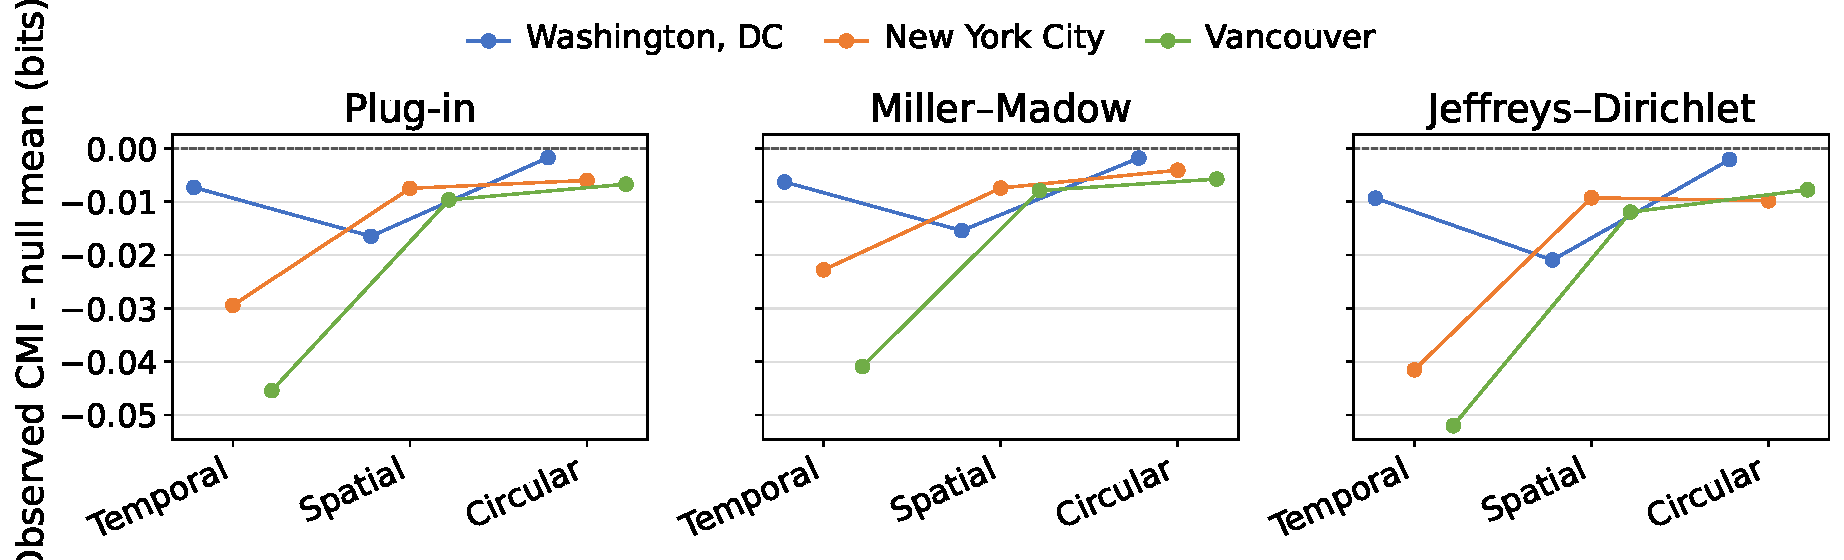
\includegraphics[width=\textwidth]{figures/e17/e17_estimator_null_sensitivity.pdf}
\caption{城市层面随机化校准的估计器敏感性。每个点表示观测 CMI 减去同一
设计条件参考分布的均值；零分布中心允许非零。}
\label{fig:sup_estimator_nulls}
\end{figure}

训练期冻结分析域敏感性比较训练期自行车服务覆盖域与完整训练期犯罪支持域。
该范围在验证和测试前已经固定，因此检验的是分析总体，而不是事后空间选择。
表~\ref{tab:sup_frozen_domain}与图~\ref{fig:sup_frozen_domain}显示，扩大空间
总体会改变 CMI 与 DELB 降幅，纽约和温哥华尤为明显。该差异属于描述性结果，
不能识别自行车因果效应。

\begin{table}[!htbp]
\begin{adjustwidth}{-\extralength}{0cm}
\caption{训练期冻结分析域敏感性。两个空间总体均在验证和测试前定义。}
\label{tab:sup_frozen_domain}
\centering
\scriptsize
\setlength{\tabcolsep}{3pt}
\begin{tabular}{llrrrrrrr}
\toprule
\textbf{城市} & \textbf{分析域} & \textbf{网格} & \textbf{$N$} & \textbf{CMI} & \textbf{$L^0$} & \textbf{$L^B$} & \textbf{$\Delta L$} & \textbf{相对下降}\\
\midrule
Washington, DC & 训练期冻结自行车覆盖域 & 181 & 198195 & 0.0432 & 0.1567 & 0.1443 & 0.0123 & 7.9\%\\
Washington, DC & 完整犯罪支持域 & 186 & 203670 & 0.0420 & 0.1535 & 0.1416 & 0.0119 & 7.7\%\\
New York City & 训练期冻结自行车覆盖域 & 198 & 216810 & 0.1314 & 0.3503 & 0.2898 & 0.0604 & 17.3\%\\
New York City & 完整犯罪支持域 & 806 & 882570 & 0.0348 & 0.1382 & 0.1288 & 0.0094 & 6.8\%\\
Vancouver & 训练期冻结自行车覆盖域 & 34 & 37230 & 0.1423 & 0.5113 & 0.4194 & 0.0919 & 18.0\%\\
Vancouver & 完整犯罪支持域 & 141 & 154395 & 0.0377 & 0.1774 & 0.1659 & 0.0115 & 6.5\%\\
\bottomrule
\end{tabular}
\end{adjustwidth}
\end{table}


\begin{figure}[!htbp]
\centering
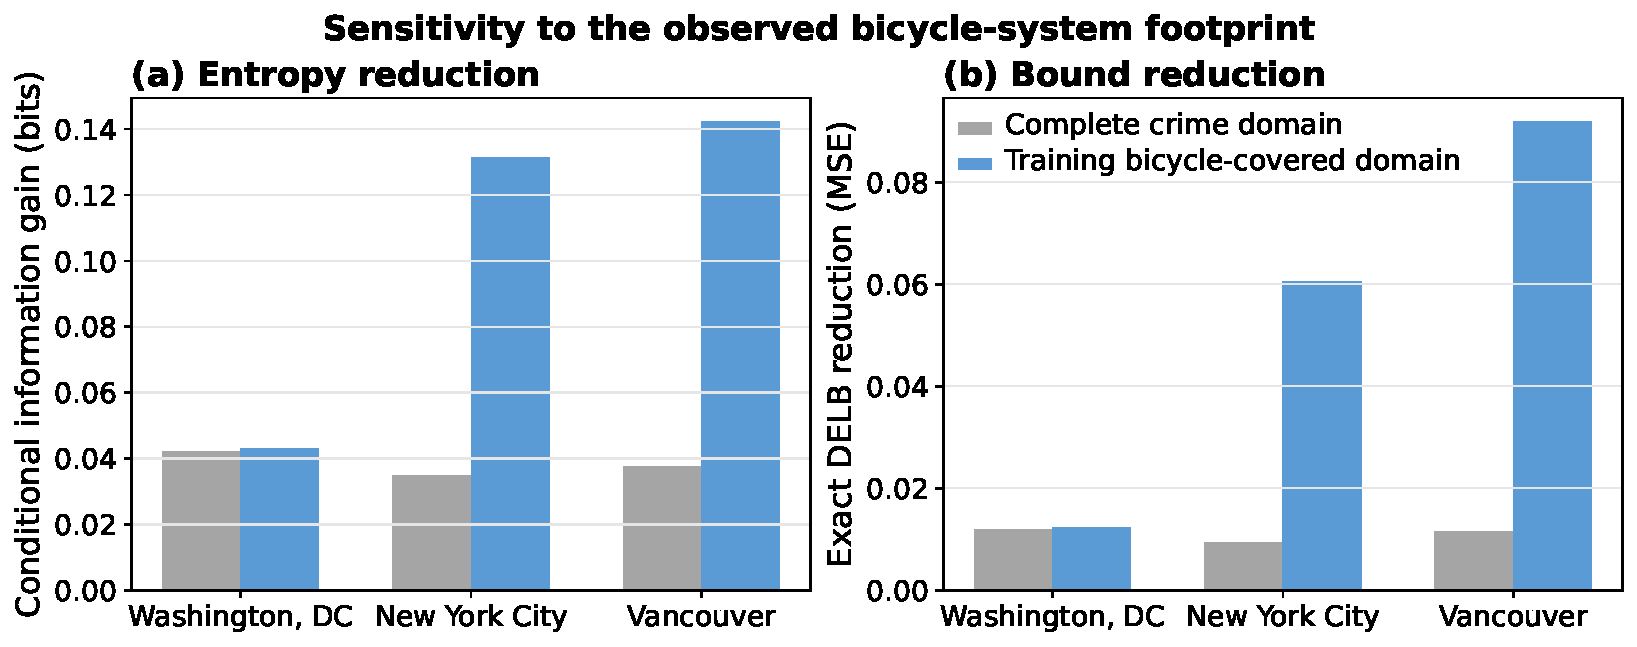
\includegraphics[width=\textwidth]{figures/e17/e04_domain_sensitivity.pdf}
\caption{训练期冻结分析域敏感性。完整犯罪支持域与训练期自行车覆盖域定义了
不同的空间目标总体。}
\label{fig:sup_frozen_domain}
\end{figure}

\section{局部估计与滞后特异性细节}
\label{supsec:moved_local_lag}


\begin{table}[H]
\caption{Spatially localized information value. The final column gives global Moran's \(I\) for DELB reduction with two-sided permutation \(p\)-values in parentheses.}
\label{tab:local_information_results}
\centering
\resizebox{\textwidth}{!}{%
\begin{tabular}{lrrrrrr}
\toprule
\textbf{City} & \textbf{Eligible/Covered} & \textbf{Median CMI} &
\textbf{Median \(\Delta L\)} & \textbf{Median \(R^L\)} &
\textbf{Positive screen} & \textbf{Moran's \(I\) (\(p\))}\\
\midrule
Washington, DC & 146/181 & 0.042 & 0.013 & 9.6\% & 137/146 & 0.164 (0.002)\\
New York City & 160/198 & 0.093 & 0.050 & 14.3\% & 155/160 & 0.038 (0.261)\\
Vancouver & 33/34 & 0.138 & 0.094 & 17.4\% & 33/33 & 0.171 (0.022)\\
\bottomrule
\end{tabular}
}
\end{table}


\begin{figure}[!htbp]
\begin{adjustwidth}{-\extralength}{0cm}
\centering
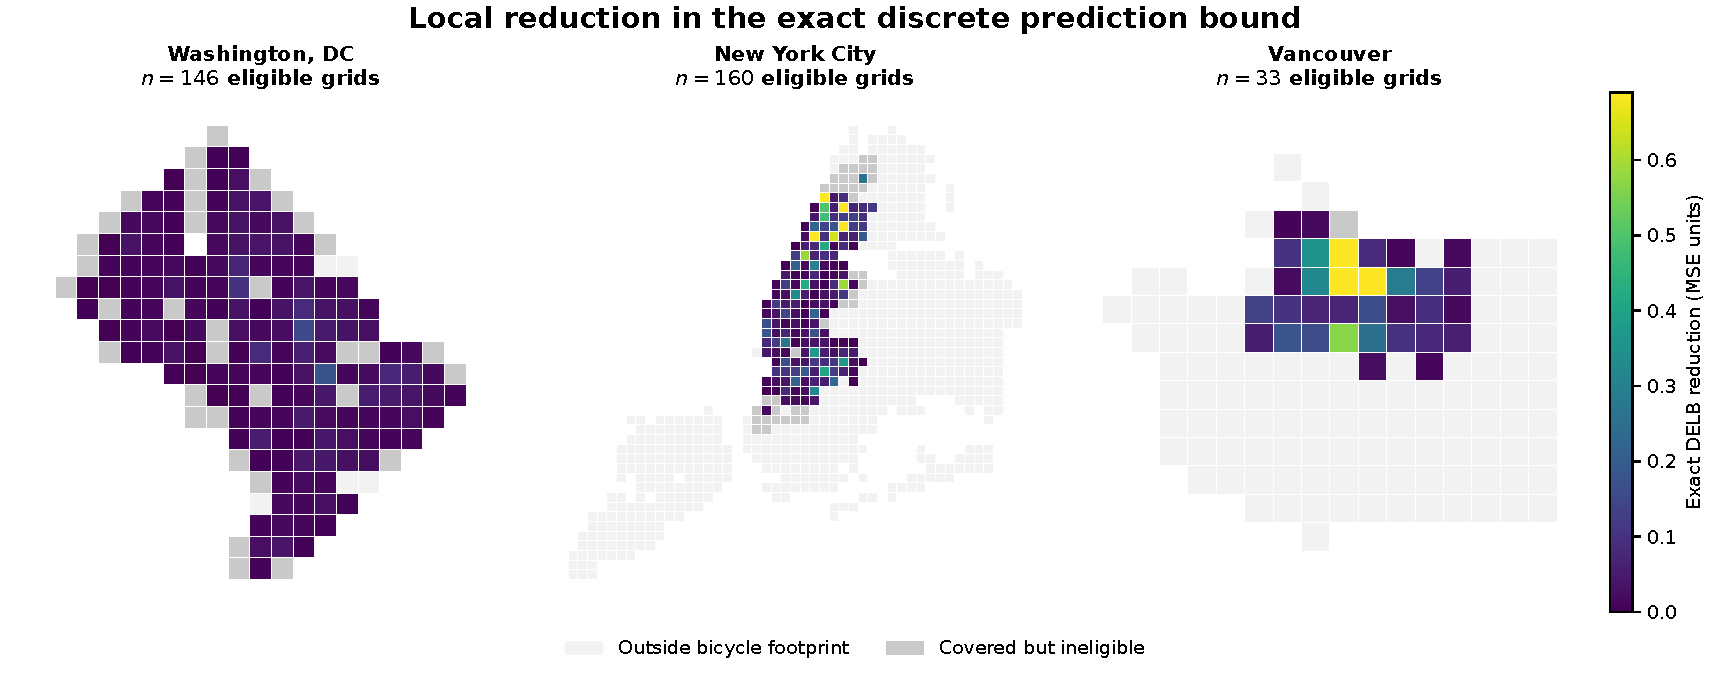
\includegraphics[width=\linewidth]{figures/e11/e05_local_delb_reduction_maps.pdf}
\end{adjustwidth}
\caption{合格网格的局部 DELB 降幅点估计。没有网格同时通过三种随机化参考。}
\label{fig:local_delb_maps}
\end{figure}

\begin{figure}[!htbp]
\centering
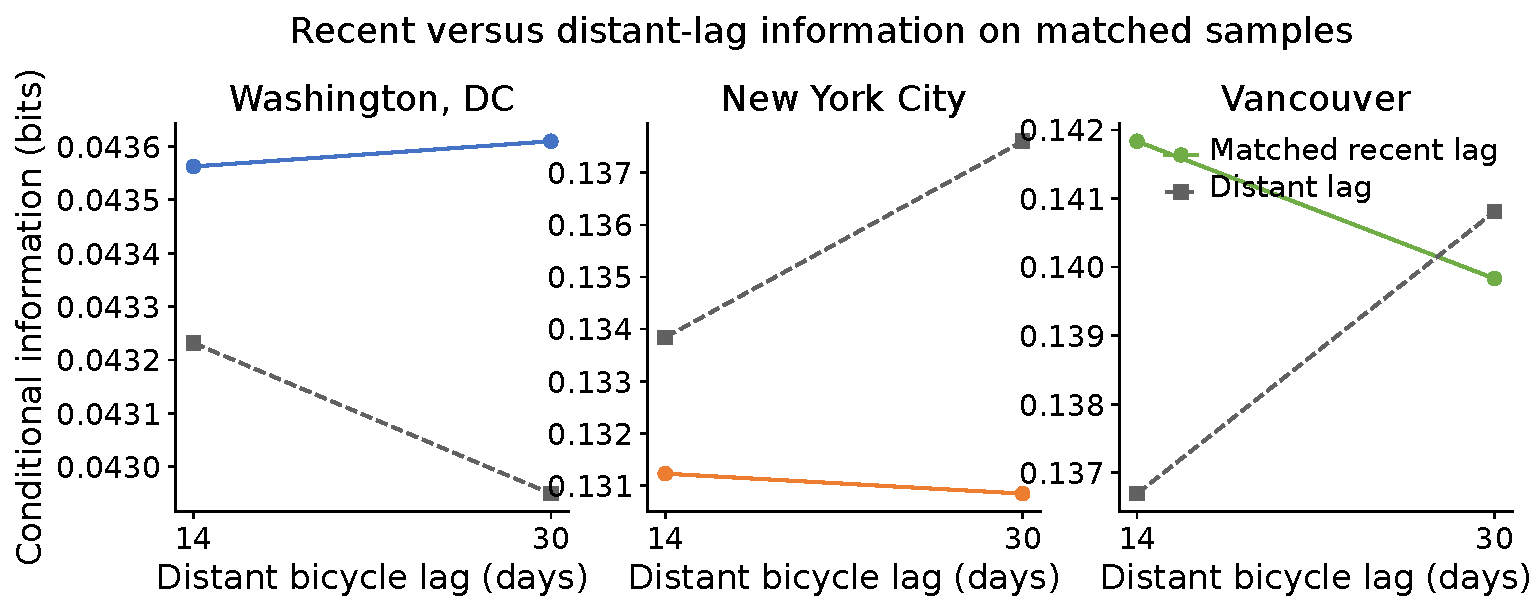
\includegraphics[width=\textwidth]{figures/e11/e10_distant_lags.pdf}
\caption{匹配的近期与远期滞后 CMI 估计。二者相近说明正的主要点估计并不特异于
一日移动时间窗。}
\label{fig:distant_lags}
\end{figure}

\section{样本量与多尺度细节}
\label{supsec:moved_scale}

\begin{table}[H]
\caption{Median relative deviation from the 100\% estimate across the 18 city--space--time cells. Quantiles over thinning repetitions are design-variability summaries, not population confidence intervals.}
\label{tab:e16_sample_stability}
\centering
\begin{tabular}{ccccc}
\toprule
\textbf{Sample fraction} & \textbf{Baseline DELB} & \textbf{Bicycle DELB} & \textbf{DELB reduction} & \textbf{CMI}\\
\midrule
20\% & 0.631 & 0.646 & 0.630 & 0.271\\
40\% & 0.423 & 0.448 & 0.341 & 0.250\\
60\% & 0.231 & 0.249 & 0.179 & 0.172\\
80\% & 0.101 & 0.114 & 0.070 & 0.087\\
100\% & 0.000 & 0.000 & 0.000 & 0.000\\
\bottomrule
\end{tabular}
\end{table}


\begin{figure}[!htbp]
\begin{adjustwidth}{-\extralength}{0cm}
\centering
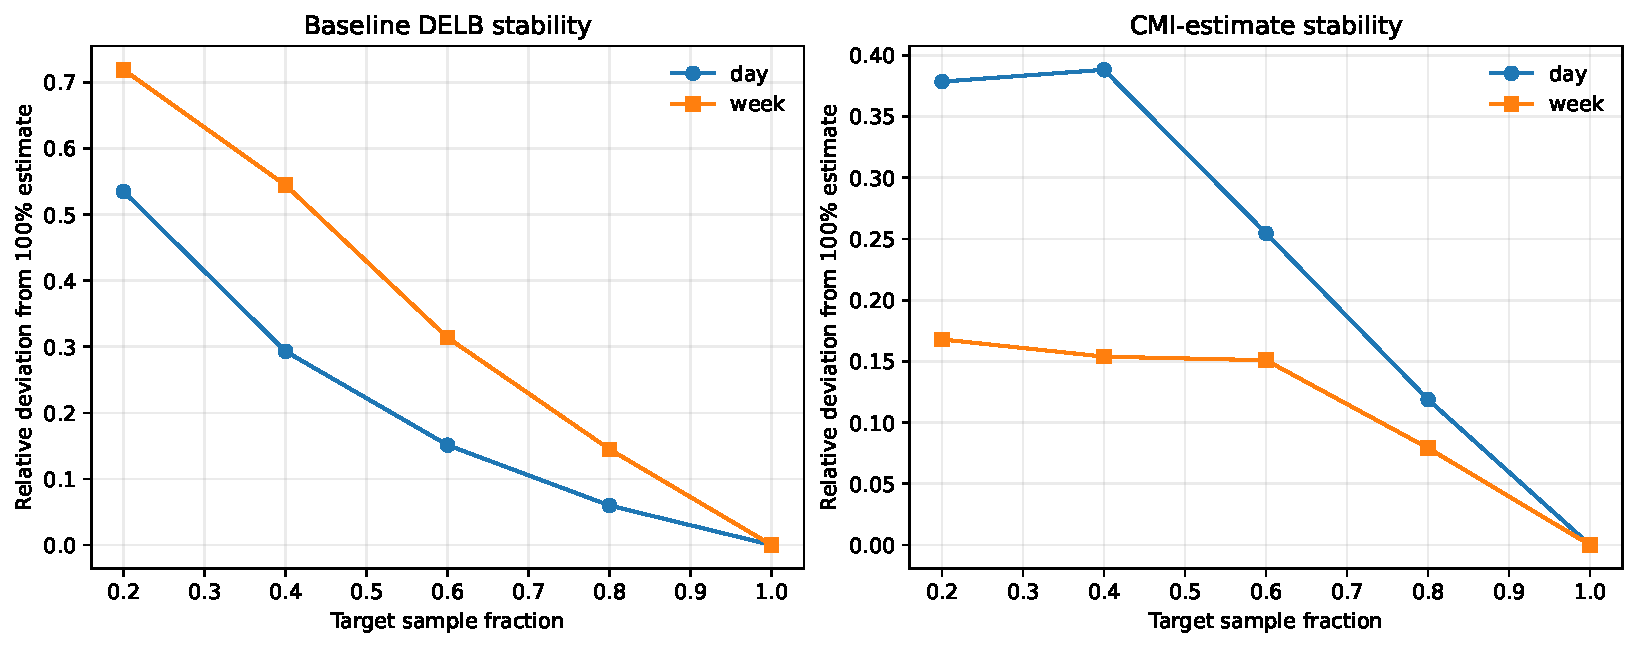
\includegraphics[width=\linewidth]{figures/e16/e16_s16_5_sample_stability.pdf}
\end{adjustwidth}
\caption{嵌套区块稀释下基线 DELB 与 CMI 估计相对完整样本的偏离。曲线衡量
估计稳定性，而非与总体真值的距离。}
\label{fig:e16_sample_stability}
\end{figure}

\begin{figure}[!htbp]
\begin{adjustwidth}{-\extralength}{0cm}
\centering
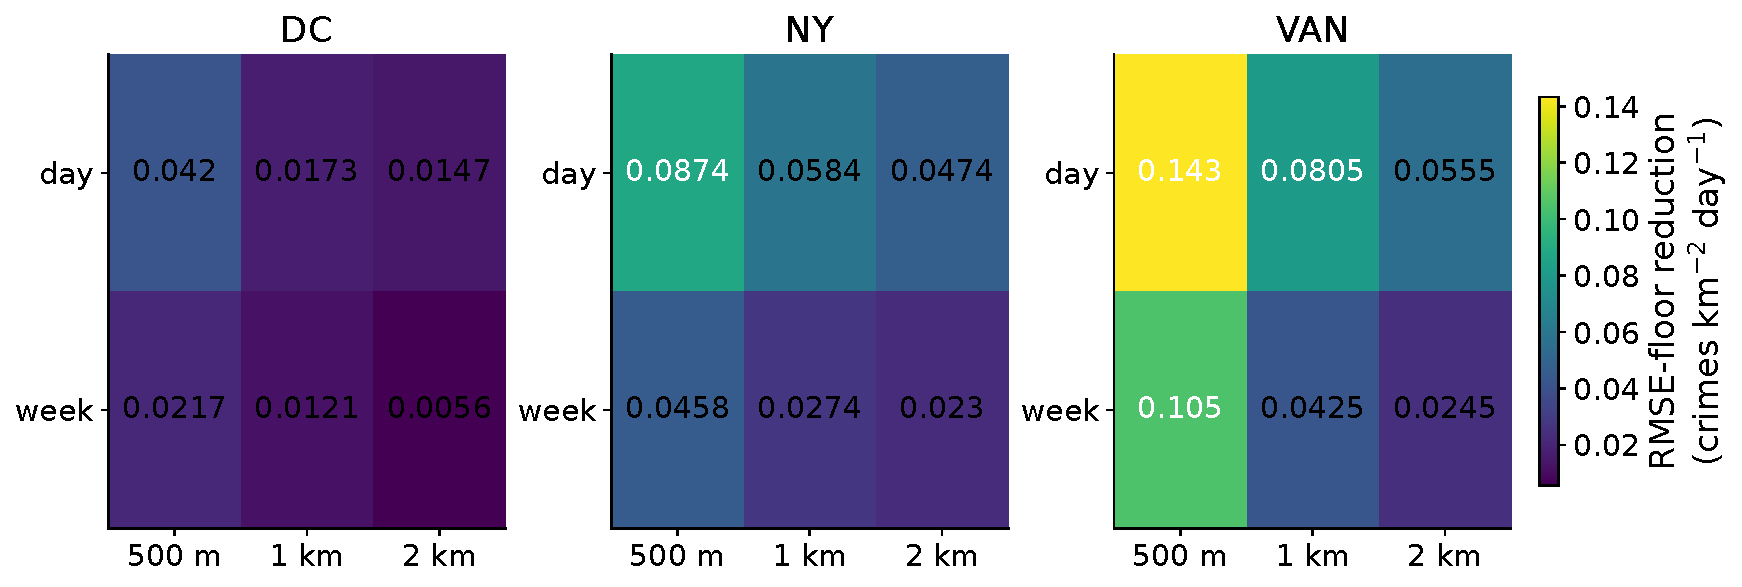
\includegraphics[width=\linewidth]{figures/e16/e16_s16_5_full_sample_intensity_heatmap.pdf}
\end{adjustwidth}
\caption{按城市、空间分辨率和时间分辨率划分的完整样本 Miller--Madow
强度 RMSE 底线下降。}
\label{fig:e16_intensity_heatmap}
\end{figure}

\begin{figure}[!htbp]
\begin{adjustwidth}{-\extralength}{0cm}
\centering
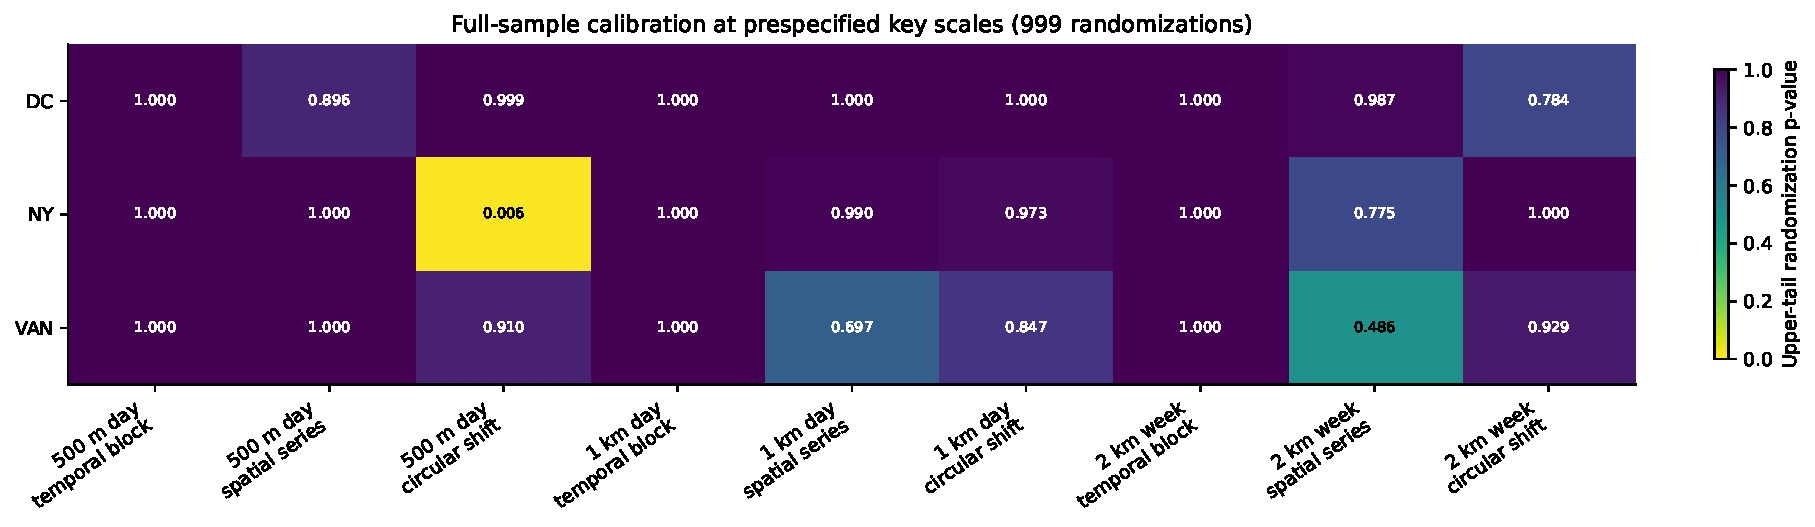
\includegraphics[width=\linewidth]{figures/e16/e16_s16_6_key_scale_pvalues.pdf}
\end{adjustwidth}
\caption{500~m--日、1~km--日和 2~km--周关键尺度的完整样本上尾随机化
\(p\) 值。}
\label{fig:e16_key_pvalues}
\end{figure}

\section{犯罪类型异质性}
\label{supsec:moved_crime_type}


\begin{table}[H]
\caption{Pooled crime-type heterogeneity in bicycle conditional information and DELB reduction. Intervals are centered 95\% seven-day block-bootstrap intervals for CMI.}
\label{tab:crime_type_heterogeneity}
\centering
\begin{tabular}{llrrrr}
\toprule
\textbf{City} & \textbf{Crime type} & \textbf{CMI} &
\textbf{95\% CI} & \(\boldsymbol{\Delta L}\) & \(\boldsymbol{R^L}\)\\
\midrule
Washington, DC & Property theft & 0.035 & [0.032, 0.038] & 0.009 & 7.1\%\\
Washington, DC & Vehicle theft & 0.012 & [0.011, 0.014] & 0.002 & 6.7\%\\
Washington, DC & Burglary & 0.006 & [0.005, 0.007] & 0.001 & 7.7\%\\
New York City & Property theft & 0.113 & [0.105, 0.121] & 0.045 & 15.8\%\\
New York City & Vehicle theft & 0.023 & [0.021, 0.025] & 0.004 & 10.1\%\\
New York City & Burglary & 0.028 & [0.026, 0.031] & 0.006 & 9.3\%\\
Vancouver & Property theft & 0.114 & [0.100, 0.128] & 0.060 & 14.9\%\\
Vancouver & Vehicle theft & 0.013 & [0.011, 0.015] & 0.002 & 8.1\%\\
Vancouver & Burglary & 0.041 & [0.034, 0.048] & 0.010 & 9.1\%\\
\bottomrule
\end{tabular}
\end{table}


\begin{figure}[!htbp]
\centering
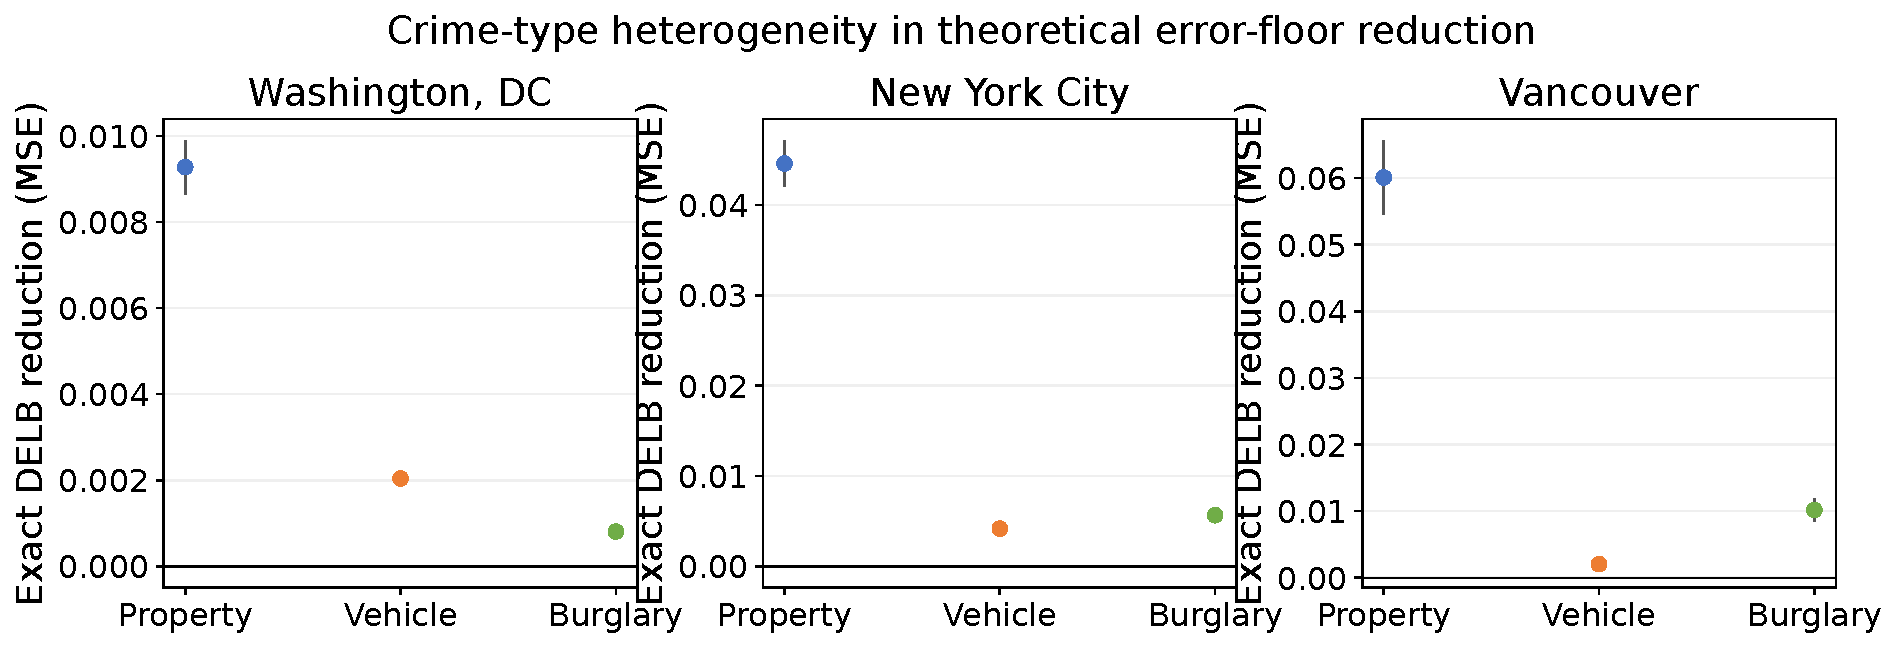
\includegraphics[width=\textwidth]{figures/e11/e08_crime_type_delb_reduction.pdf}
\caption{按统一犯罪类别和城市划分的 DELB 降幅点估计。区间表示区块 bootstrap
抽样变异，不是类别特异随机化检验。}
\label{fig:crime_type_delb}
\end{figure}

\section{替代规格与滚动起点}
\label{supsec:moved_rolling}


\begin{table}[H]
\caption{Robustness summary across information specifications and rolling forecasts. Positive theory specifications count
Miller--Madow DELB reductions across 16 pre-specified alternatives.
Rolling forecasts comprise 12 monthly origins for each of four model
families. Positive \(\Delta\mathrm{MSE}\) favors the bicycle-aware model.}
\label{tab:robustness_summary}
\begin{adjustwidth}{-\extralength}{0cm}
\centering
\resizebox{\linewidth}{!}{%
\begin{tabular}{lrrrrrr}
\toprule
\textbf{City} & \textbf{Positive theory} & \textbf{Positive origins} &
\multicolumn{2}{c}{\textbf{State mean}} &
\multicolumn{2}{c}{\textbf{Gradient boosting}}\\
\cmidrule(lr){4-5}\cmidrule(lr){6-7}
 & & & \textbf{Positive} & \textbf{Mean \(\Delta\)MSE} &
\textbf{Positive} & \textbf{Mean \(\Delta\)MSE}\\
\midrule
Washington, DC & 16/16 & 23/48 & 66.7\% & 0.001 & 41.7\% & 0.000\\
New York City & 16/16 & 26/48 & 91.7\% & 0.030 & 100.0\% & 0.076\\
Vancouver & 16/16 & 20/48 & 66.7\% & 0.006 & 41.7\% & -0.006\\
\bottomrule
\end{tabular}
}
\end{adjustwidth}
\end{table}


\begin{figure}[!htbp]
\begin{adjustwidth}{-\extralength}{0cm}
\centering
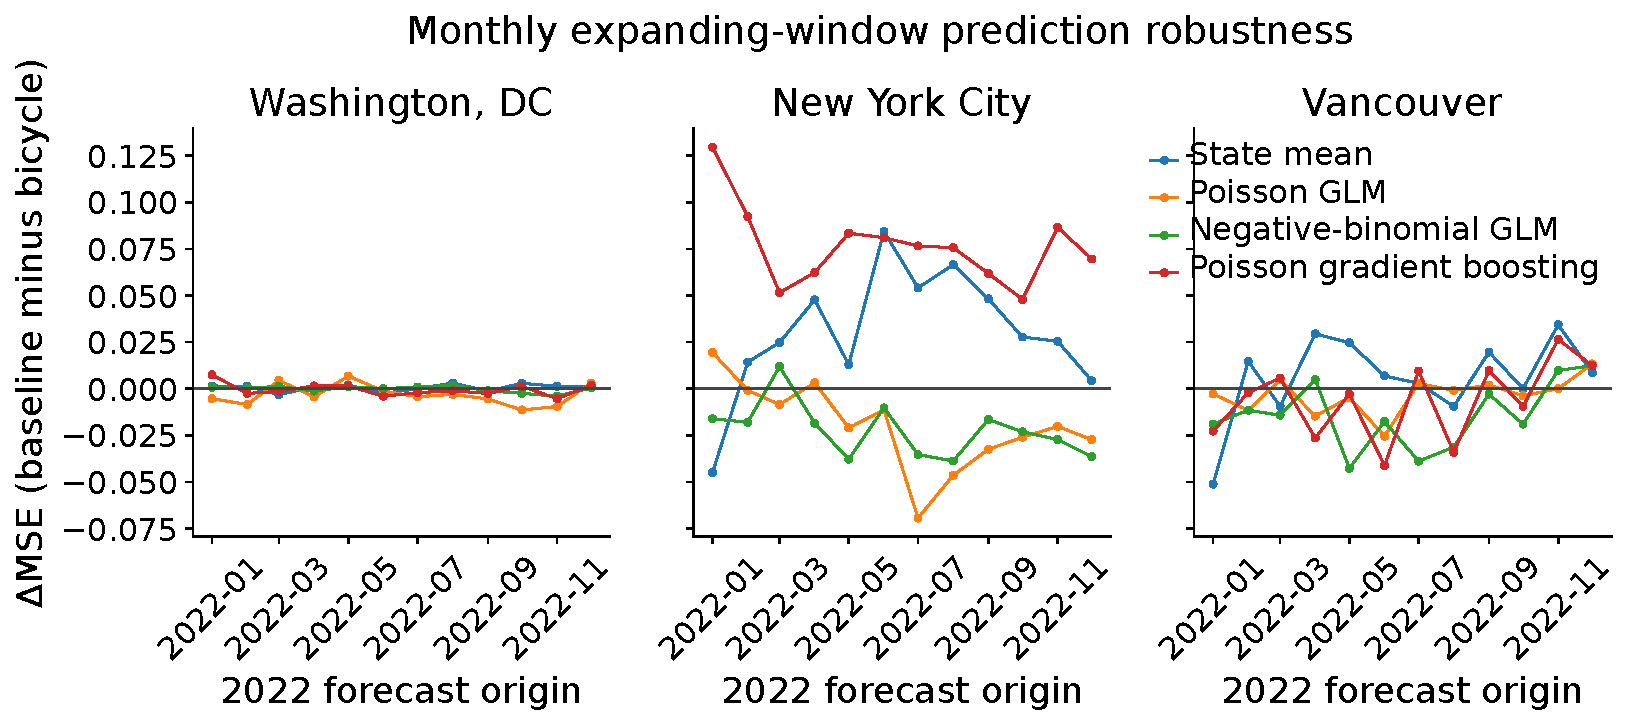
\includegraphics[width=\linewidth]{figures/e11/e09_rolling_origins.pdf}
\end{adjustwidth}
\caption{扩展窗口月度预测结果。正的 \(\Delta\mathrm{MSE}\) 有利于自行车增强
模型；稳定性仍然取决于模型。}
\label{fig:rolling_origins}
\end{figure}

\section{其他描述性与有限样本图}
\label{supsec:additional_figures}

图~\ref{fig:spatial_patterns}和图~\ref{fig:monthly_patterns}属于描述性审计。
它们尚未进行条件化，因此不构成 CMI、DELB 下降或移动因果效应的证据。

\begin{figure}[!htbp]
\begin{adjustwidth}{-\extralength}{0cm}
\centering
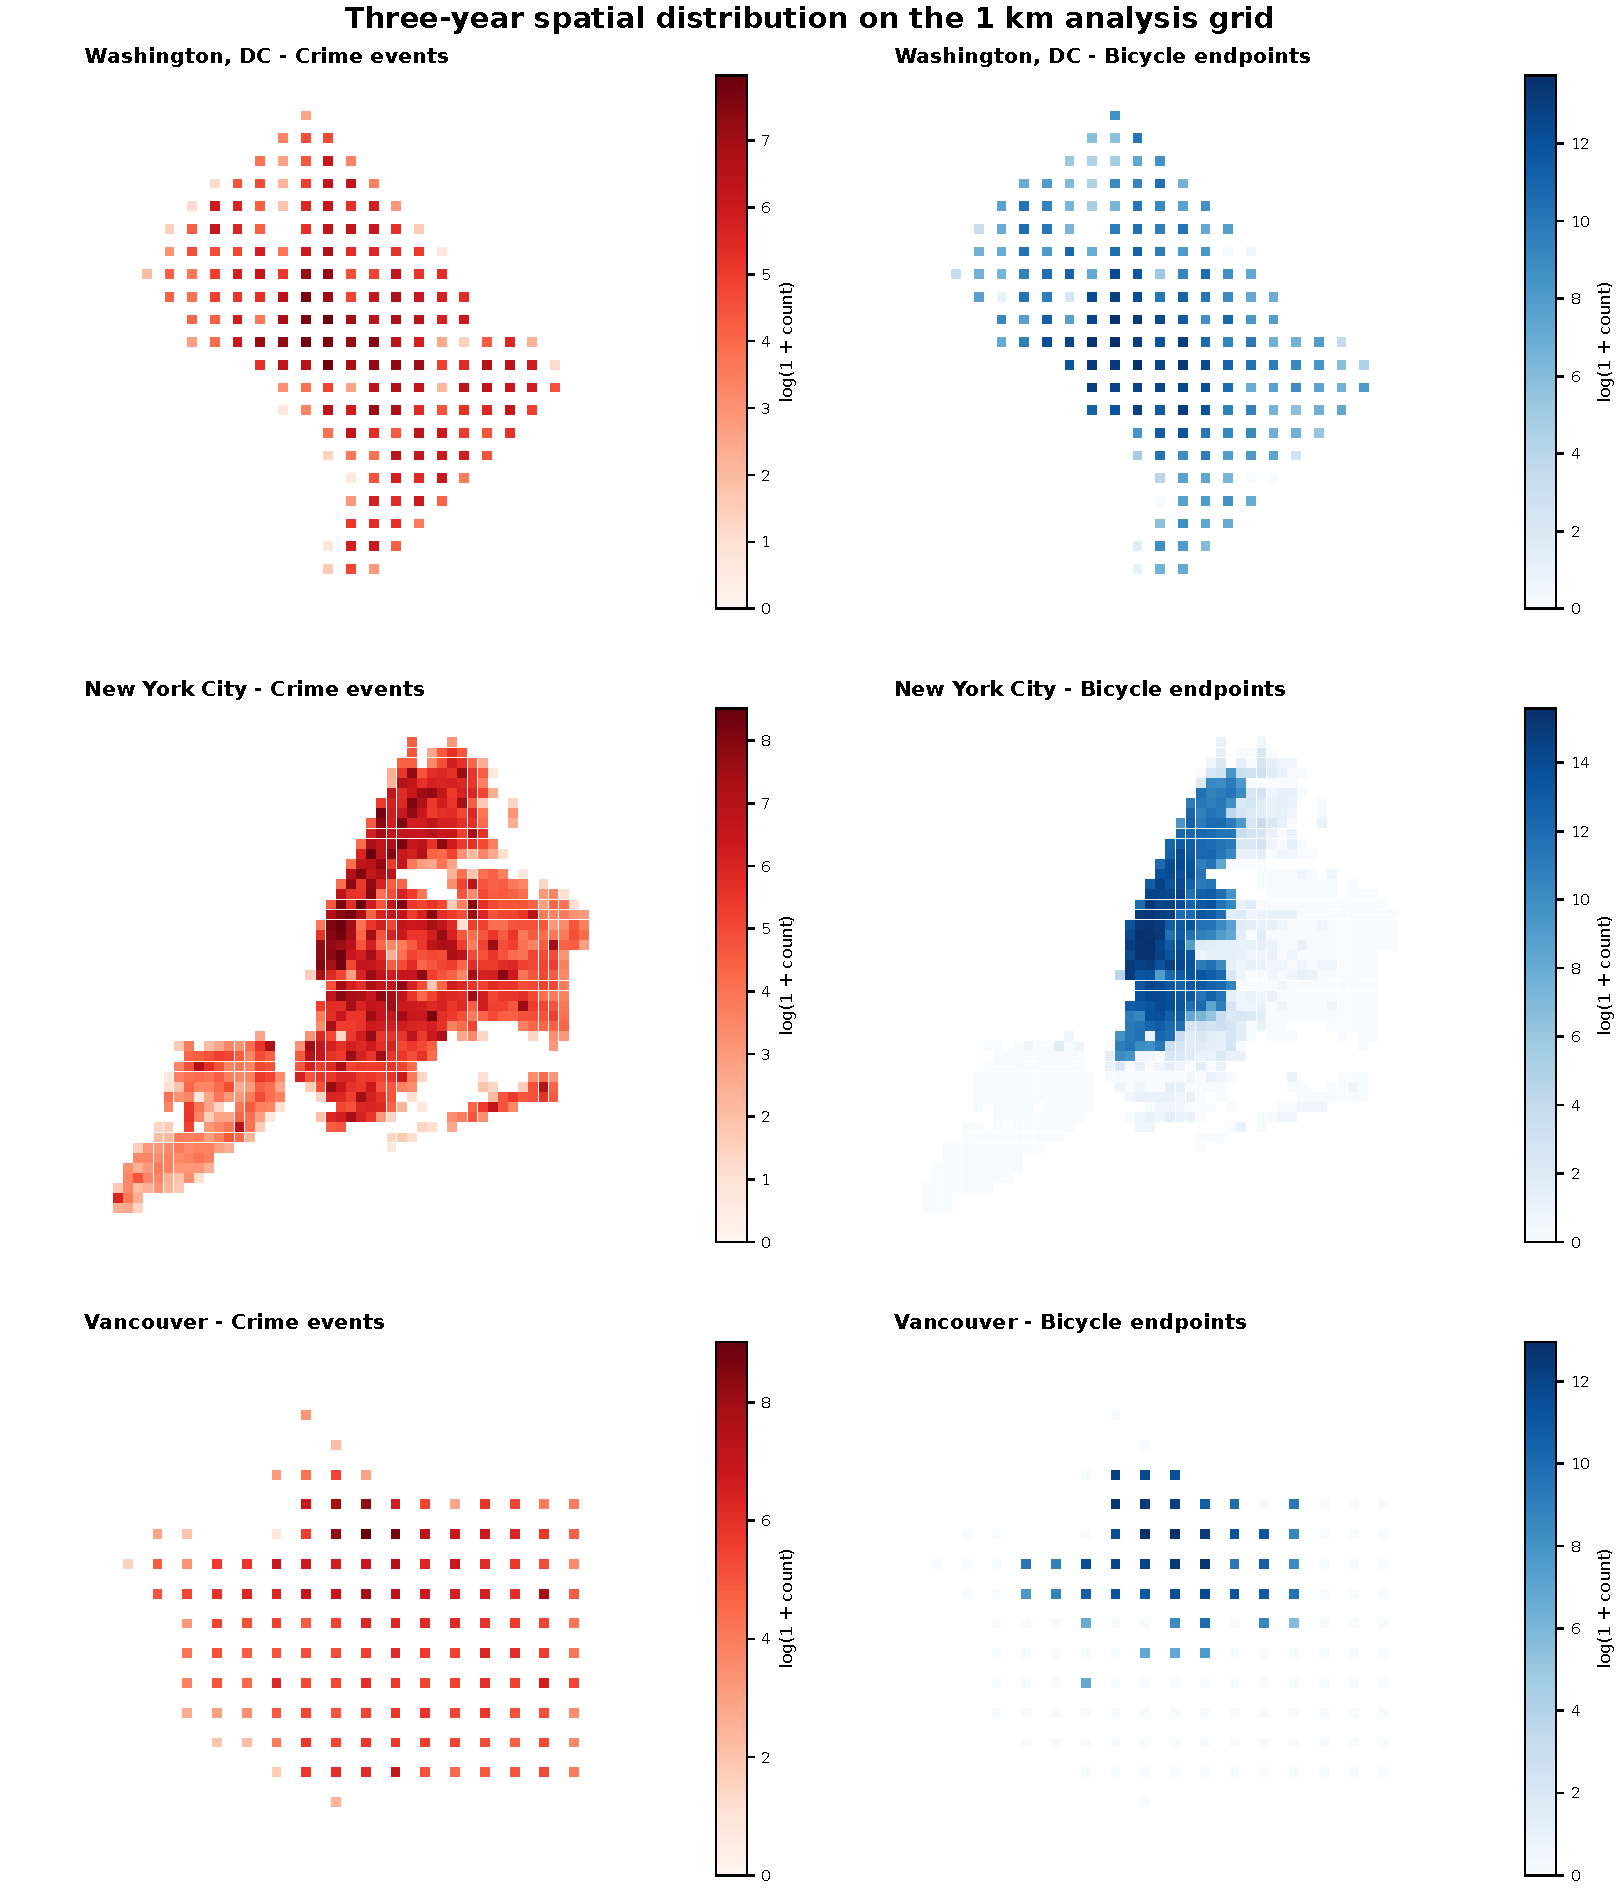
\includegraphics[width=0.98\linewidth]{figures/e11/e02_spatial_patterns.pdf}
\end{adjustwidth}
\caption{2020--2022 年统一财产犯罪计数与自行车端点流量的空间集中度。}
\label{fig:spatial_patterns}
\end{figure}

\begin{figure}[!htbp]
\centering
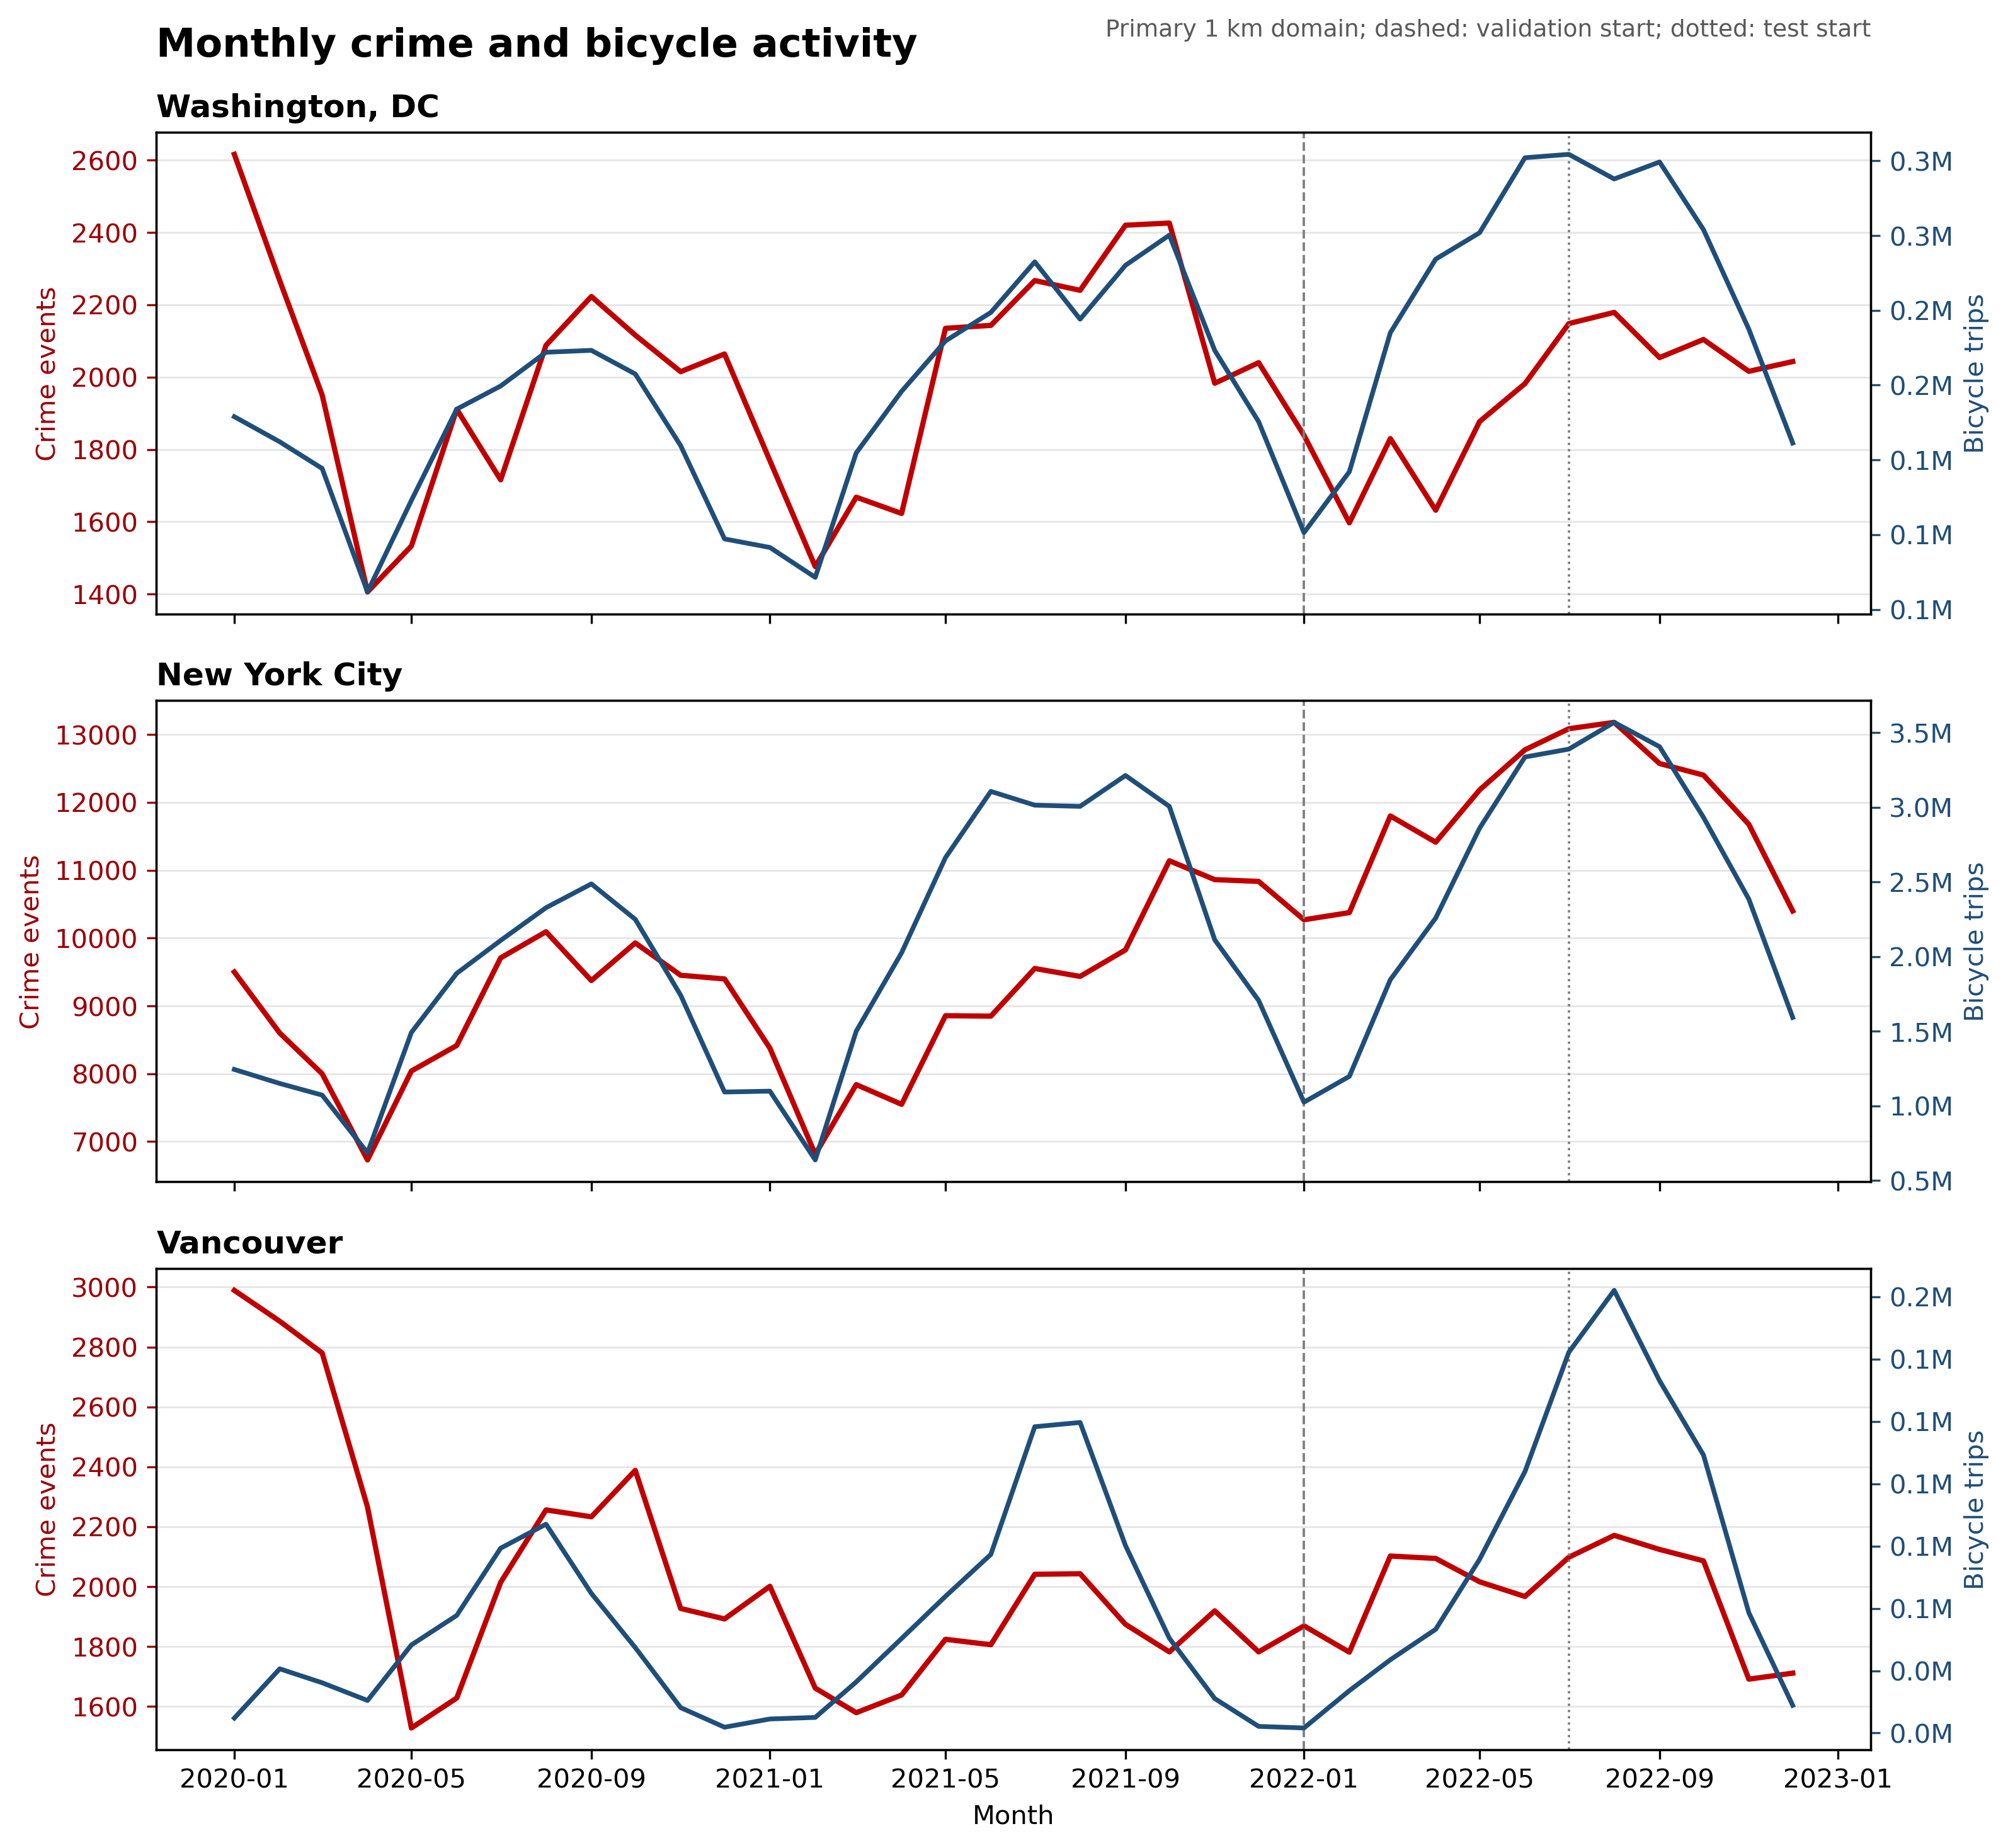
\includegraphics[width=\textwidth]{figures/e11/e02_monthly_patterns.png}
\caption{2020--2022 年各城市月度犯罪计数与自行车端点流量。}
\label{fig:monthly_patterns}
\end{figure}

\begin{figure}[!htbp]
\begin{adjustwidth}{-\extralength}{0cm}
\centering
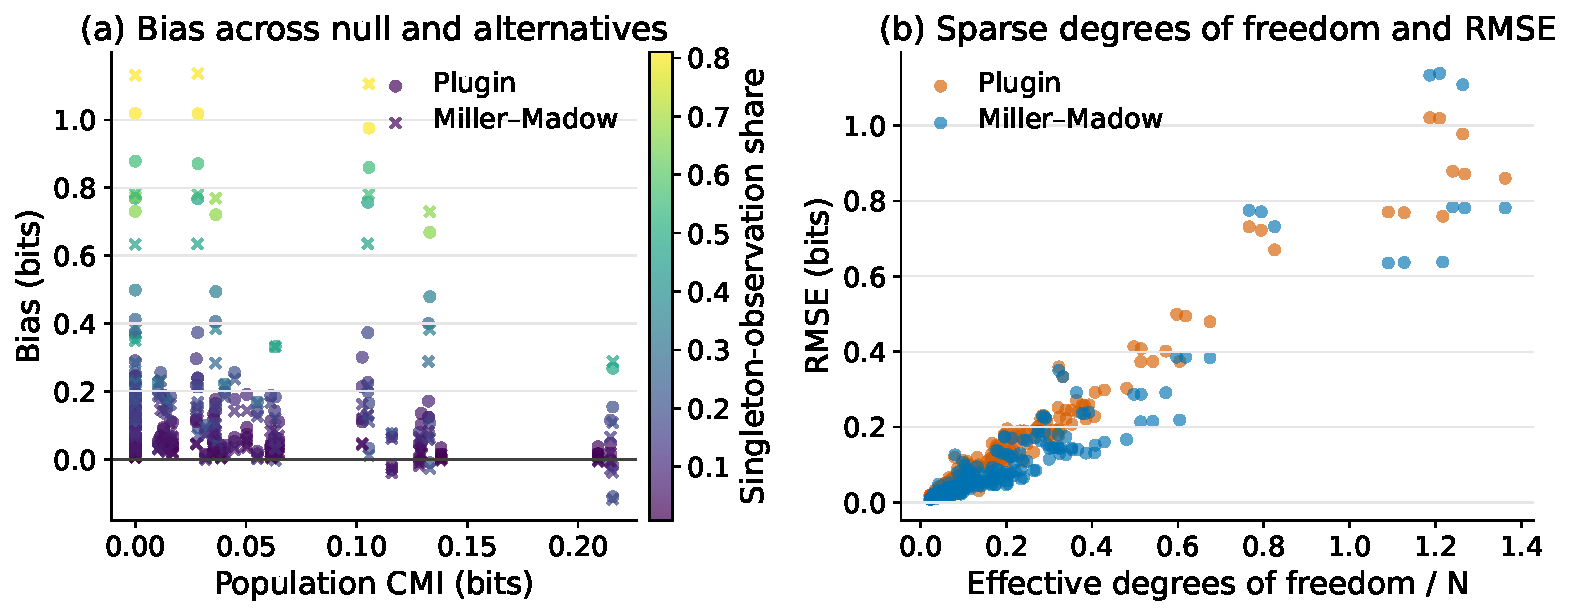
\includegraphics[width=\linewidth]{figures/s7/e12_bias_rmse_supplement.pdf}
\end{adjustwidth}
\caption{完整稀疏状态模拟网格中的估计偏差与 RMSE。}
\label{fig:e12_bias_supplement}
\end{figure}

\begin{figure}[!htbp]
\begin{adjustwidth}{-\extralength}{0cm}
\centering
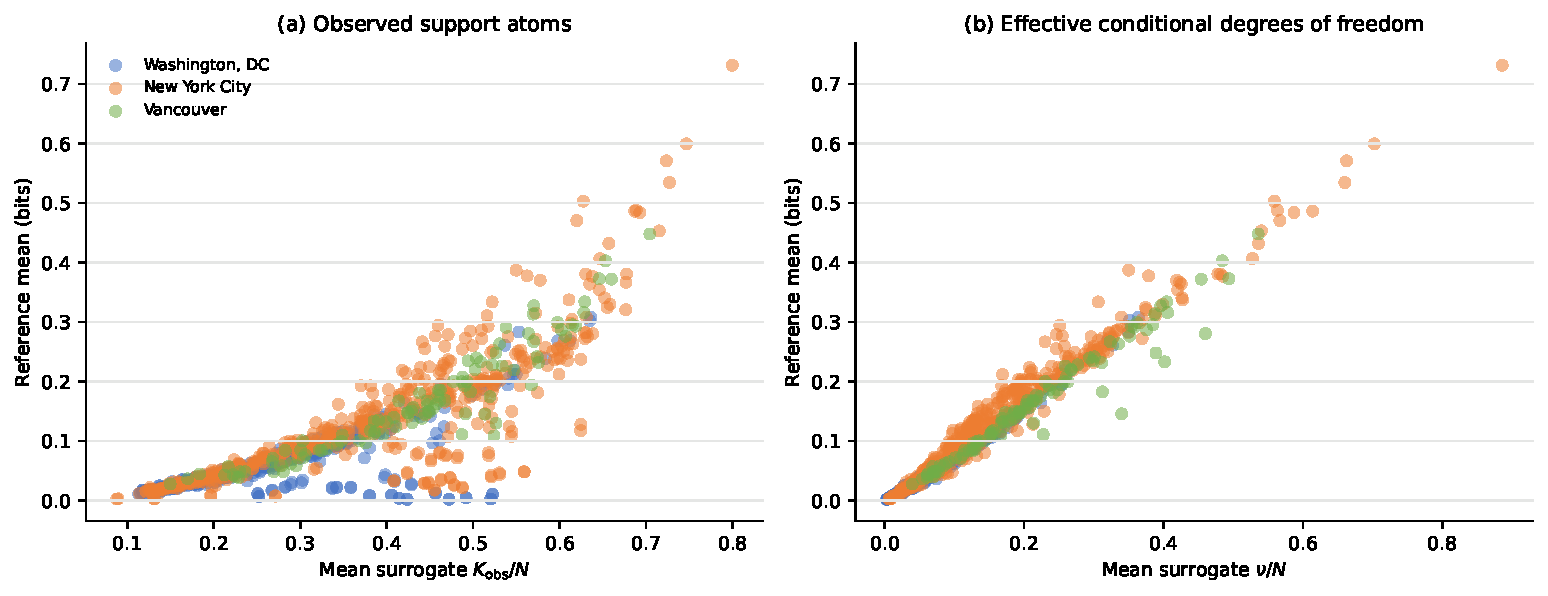
\includegraphics[width=\linewidth]{figures/s7/e13_support_metrics_supplement.pdf}
\end{adjustwidth}
\caption{模拟和经验零分布汇总中的支持度指标关系。}
\label{fig:e13_support_supplement}
\end{figure}

\begin{figure}[!htbp]
\begin{adjustwidth}{-\extralength}{0cm}
\centering
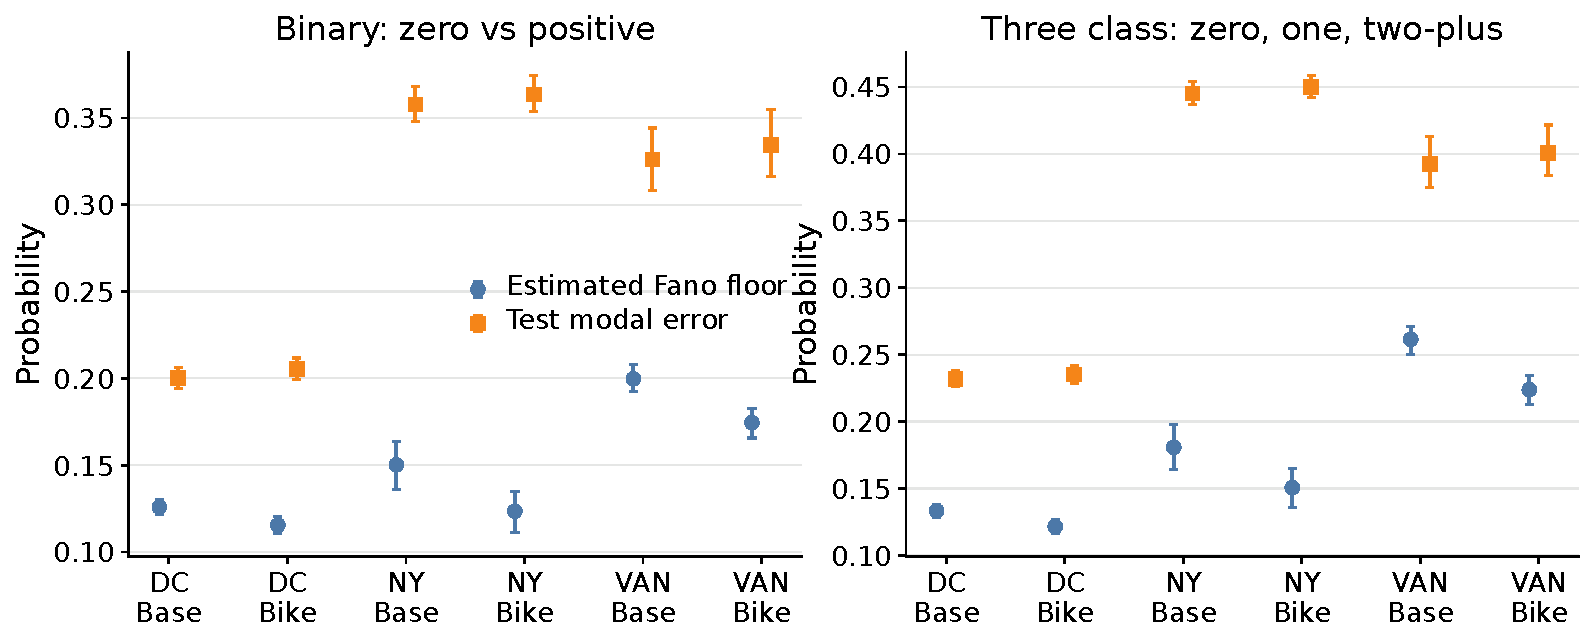
\includegraphics[width=\linewidth]{figures/s7/e14_fano_bootstrap.pdf}
\end{adjustwidth}
\caption{估计 Fano 底线与留出众数分类器误差的中心化七日区块 bootstrap 区间。}
\label{fig:e14_bootstrap_supplement}
\end{figure}
